\documentclass[a4paper, 12pt]{article}
%\usepackage{enumerate}
\usepackage{graphicx}
\usepackage[utf8]{vietnam} 
\usepackage{amsmath}
\usepackage{hyperref}
\hypersetup{
    colorlinks=true,
    linkcolor=blue,
    filecolor=magenta,      
    urlcolor=cyan,
}
\usepackage{makecell}
\usepackage{caption}
\usepackage{tabularx}
\title{CTT451 - Báo cáo cuối kỳ \\ Nhận diện cử chỉ tay}
\date{\today}

\begin{document}

\begin{center} 
\large VNUHCM - Khoa học tự nhiên \\
Công nghệ thông tin \\
Chương trình chất lượng cao \\
\end{center}
\begingroup
\let\newpage\relax
\maketitle
\endgroup
\textbf{Thành viên nhóm:}
\begin{enumerate}
	\item 1453058: Trần Sơn Vũ
	\item 1453034: Huỳnh Thiên Phước
\end{enumerate}

\section{Tổng quan}
Trong xa hội hiện nay việc giao tiếp giữa người bình thường và người khuyết tật nói chung và người mất khả năng nghe nói riêng còn gặp nhiều khó khăn. Chính vì vậy chúng tôi đã nghiên cứu và thử nghiệm để giải quyết được những bước đầu của vấn đề này, đó là nhận diện cử chỉ của 1 bàn tay. Nghiên cứu của chúng tôi như sau: khi một người đứng trước camera thể hiện thủ ngữ bất kì thì nó sẽ trả về ký tự trong bảng chữ cái nhưng trong nghiên cứu này chúng tôi sẽ chỉ trả về số từ 1 đến 5.
\begin{figure}[!ht]
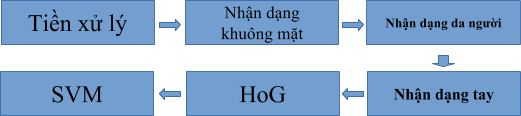
\includegraphics[width=\textwidth]{overview.png}
\caption{Hệ thống nhận diện cử chỉ tay}
\label{fig:overview}
\end{figure}
\section{Phương pháp luận}
Chúng tôi sẽ thực hiện những bước như sau theo hình \ref{fig:overview}: Đầu tiên, khi nhận được dữ liệu đầu vào từ camera chúng tôi sẽ loại nhiễu ảnh. Bước tiếp theo chúng tôi nhận diện khuôn mặt(để phân biệt khuôn mặt với tay người). Sau đó, nhận dạng da người trong ảnh rồi so sánh với khuôn mặt đã nhận dạng trước đó để loại bỏ nó. Sau đó áp dụng HoG để tạo vector đặc trưng, bỏ vào SVM để cho ra kết quả.
\subsection{Tiền xử lý}
Áp dụng bộ lọc Gaussian theo công thức $G_{0}(x, y) = A e^{ \dfrac{ -(x - \mu_{x})^{2} }{ 2\sigma^{2}_{x} } + \dfrac{ -(y - \mu_{y})^{2} }{ 2\sigma^{2}_{y} } }$ để làm mờ ảnh và loại bỏ nhiễu.
\subsection{Nhận dạng khuôn mặt }
Chúng tôi áp dụng nhận dạng khuôn mặt cơ bản của OpenCV là Haar Feature-based Cascade Classifiers. Để chương trình xử lý nhanh chúng tôi giả định chỉ có một người trước camera. vì vậy chúng tôi chỉ lấy khuôn mặt lớn nhất và phải có kích thước lớn hơn một ngưỡng mà chúng tôi đã xét trong tất cả các khuôn mặt mà nó nhận dang được.
Mục đích dùng nhận diện khuôn mặt vì camera quay trúng khuôn mặt, và bàn tay sẽ gây nhiễu kết quả, không phân biệt được tay người và khuôn mặt. 
\subsection{Nhận dạng màu da}
Đầu tiên chúng tôi chuyển ảnh từ RGB sang HSV vì HSV cho chúng ta biết: H(Hue, vùng màu), S(Saturation, độ bão hòa màu), V(Value, độ sáng) sẽ giúp chúng ta dễ dàng lọc được màu từ ảnh. Để có thể tìm được ngưỡng màu phù hợp để có thể tách được da người từ ảnh đầu vào, bằng phương pháp thực nghiệm thử và sai chúng tôi đã tìm ra được thông số mà phù hợp với người Việt Nam nói riêng và người da vàng nói chung. Thông số chúng tôi sử dụng trong ngưỡng từ (0, 10, 60) đến (20, 150, 255).
\subsection{Nhận dạng tay}
Sau khi đã nhận dạng da người chúng tôi phát hiện ra rằng nếu nhận dạng màu da thì có thể lấy cả mặt người vì vậy chúng tôi đã nhận dạng mặt người để có thể loại bỏ mặt người ra khỏi ảnh bằng cách lấy giá trị của từng pixel mặt người thành giá trị 0 trong ảnh mà chúng tôi đã tách từ da người. Chúng ta dùng contours để xác định vùng tay và cắt nó ra. Thêm vào đó để xử lý nhanh chúng tôi tiếp tục giả định chỉ có một cánh tay vì vậy chúng tôi sẽ lấy vùng có diện tích lớn nhất và có diện tích lớn hơn một ngưỡng mà chúng tôi đã xét trong các vùng coutours đã tìm được. Để tăng độ chính xác chúng tôi đã sử dụng 1 vòng tay màu đen để dễ dàng phân biệt được giữa bàn tay với cánh tay.
\subsection{HoG}
Tiếp theo, chúng tôi sẽ đi tìm vector đặc trưng của contours đã tách bằng phương pháp HoG qua những bước sau: Đầu tiên chúng tôi sẽ chuyển sang grayscale và scale ảnh lại với kích thước là 32 x 32 để có thể tổng quát hóa kích thước của tất cả các ảnh có kích thước như nhau cho việc so sánh sau này. Sau đó lấy ảnh đó tính gradiant theo x và y bằng cách sử dụng tích chập $G_{x} = D_{x} * I$ và $G_{y} = D_{y} *I $ với I là hình ảnh đầu vào, $D_{x}$ là bộ lọc cho chiều x, và $D_{y}$ là bộ lọc cho chiều y. Trong đồ án này, chúng tôi sẽ sử dụng Sobel để tính với Dx và Dy với công thức là $D_{x} =  \begin{bmatrix} -1 & 0 & +1 \\ -2 & 0 & +2 \\ -1 & 0 & +1 \end{bmatrix}$ và $D_{y} =  \begin{bmatrix} -1 & 0 & +1 \\ -2 & 0 & +2 \\ -1 & 0 & +1 \end{bmatrix}$. Khi đã có được Gx và Gy cho mỗi pixel, chúng tôi sẽ tìm độ lớn và hướng của gradiant bằng công thức sau $G = \sqrt{G^2_x + G^2_y}$ và $\theta = \arctan \frac{G_y}{G_x}$. Kế tiếp chúng tôi chia ảnh thành 4 x 4 cells và tính histogram of gradients cho từng cell. Chúng tôi sử dụng 8 bins theo thứ tự 0, 45, 90, 135, 180, 225, 270, 315. Chúng tôi sẽ xem góc gradiant của mỗi pixel sẽ thuộc bin gần nhất nào rồi cộng độ lớn cho bin đó. Sau đó chúng tôi sẽ gộp thành vector rồi tính normalize của nó để lọc nhiễu ánh sáng. Cuối cùng chúng tôi sẽ được 1 vector có 128 đặc trưng.

\subsection{SVM}
Chúng tôi sử dụng SVM tuyến tính để có thể cho tốc độ xử lý nhanh thì mới có thể phù hợp với chương trình real time quay xử lý trực tiếp như chương trình chúng tôi. 
\section{Dữ liệu train}
Chúng tôi đã sử dụng dữ liệu từ trang web \url{http://www-vpu.eps.uam.es/DS/HGds/} này để train. Và chúng tôi chỉ sử dụng 5 mẫu của bản tay biểu diễn từ số 1 đến 5, mỗi mẫu chúng tôi lấy khoảng 200 tấm hình. Mỗi tấm hình đều là hình ảnh grayscale với bàn tay kích thước nhỏ nằm tại chính giữa ảnh. Vấn đề đặt ra là phải cắt được bàn tay để có thể tăng được độ chính xác. Các bước mà chúng tôi xử lý vấn đề trên như sau: do hình ảnh đãủa là grayscale và chất lượng tương đối tốt nên không cần bước loại nhiễu. Vì vậy ngay bước đầu chúng tôi tìm contours của bàn tay để có thể tách được một hình chữ nhật bao phủ bàn tay, cuối cùng scale ảnh về kích thước 32x32, kích thước do chúng tôi quy định như ở phần trước. Sau đó sẽ bỏ vào HoG và đánh label từng ảnh. Cuối cùng train tất cả ảnh bằng SVM.
\section{Kết quả}
Đây là \href{https://www.youtube.com/watch?v=jdHNLqCSJrM&feature=youtu.be}{kết quả} mà chúng tôi thu được:
\begin{figure}[!ht]
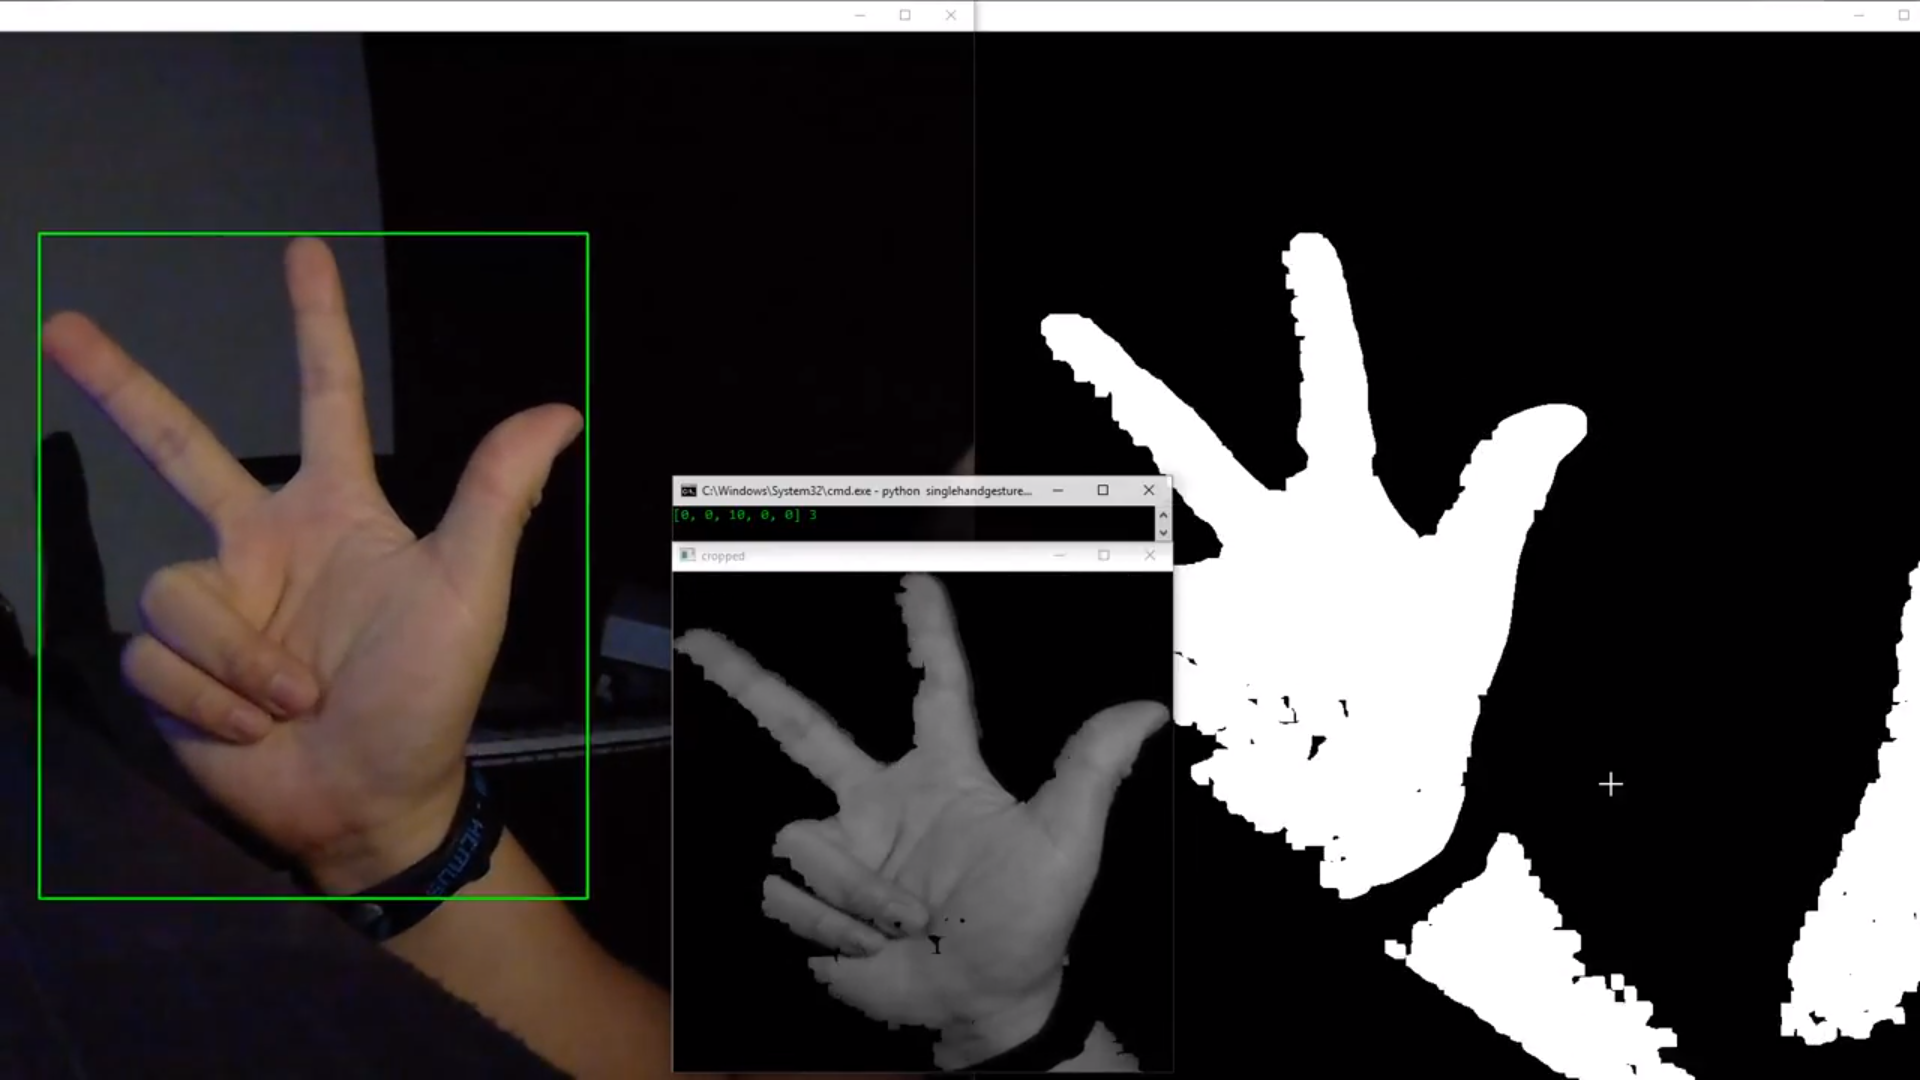
\includegraphics[width=\textwidth]{result_1.png}
\caption{Kết quả khi đưa 3 ngón tay}
\label{fig:foo}
\end{figure}

\begin{figure}[!ht]
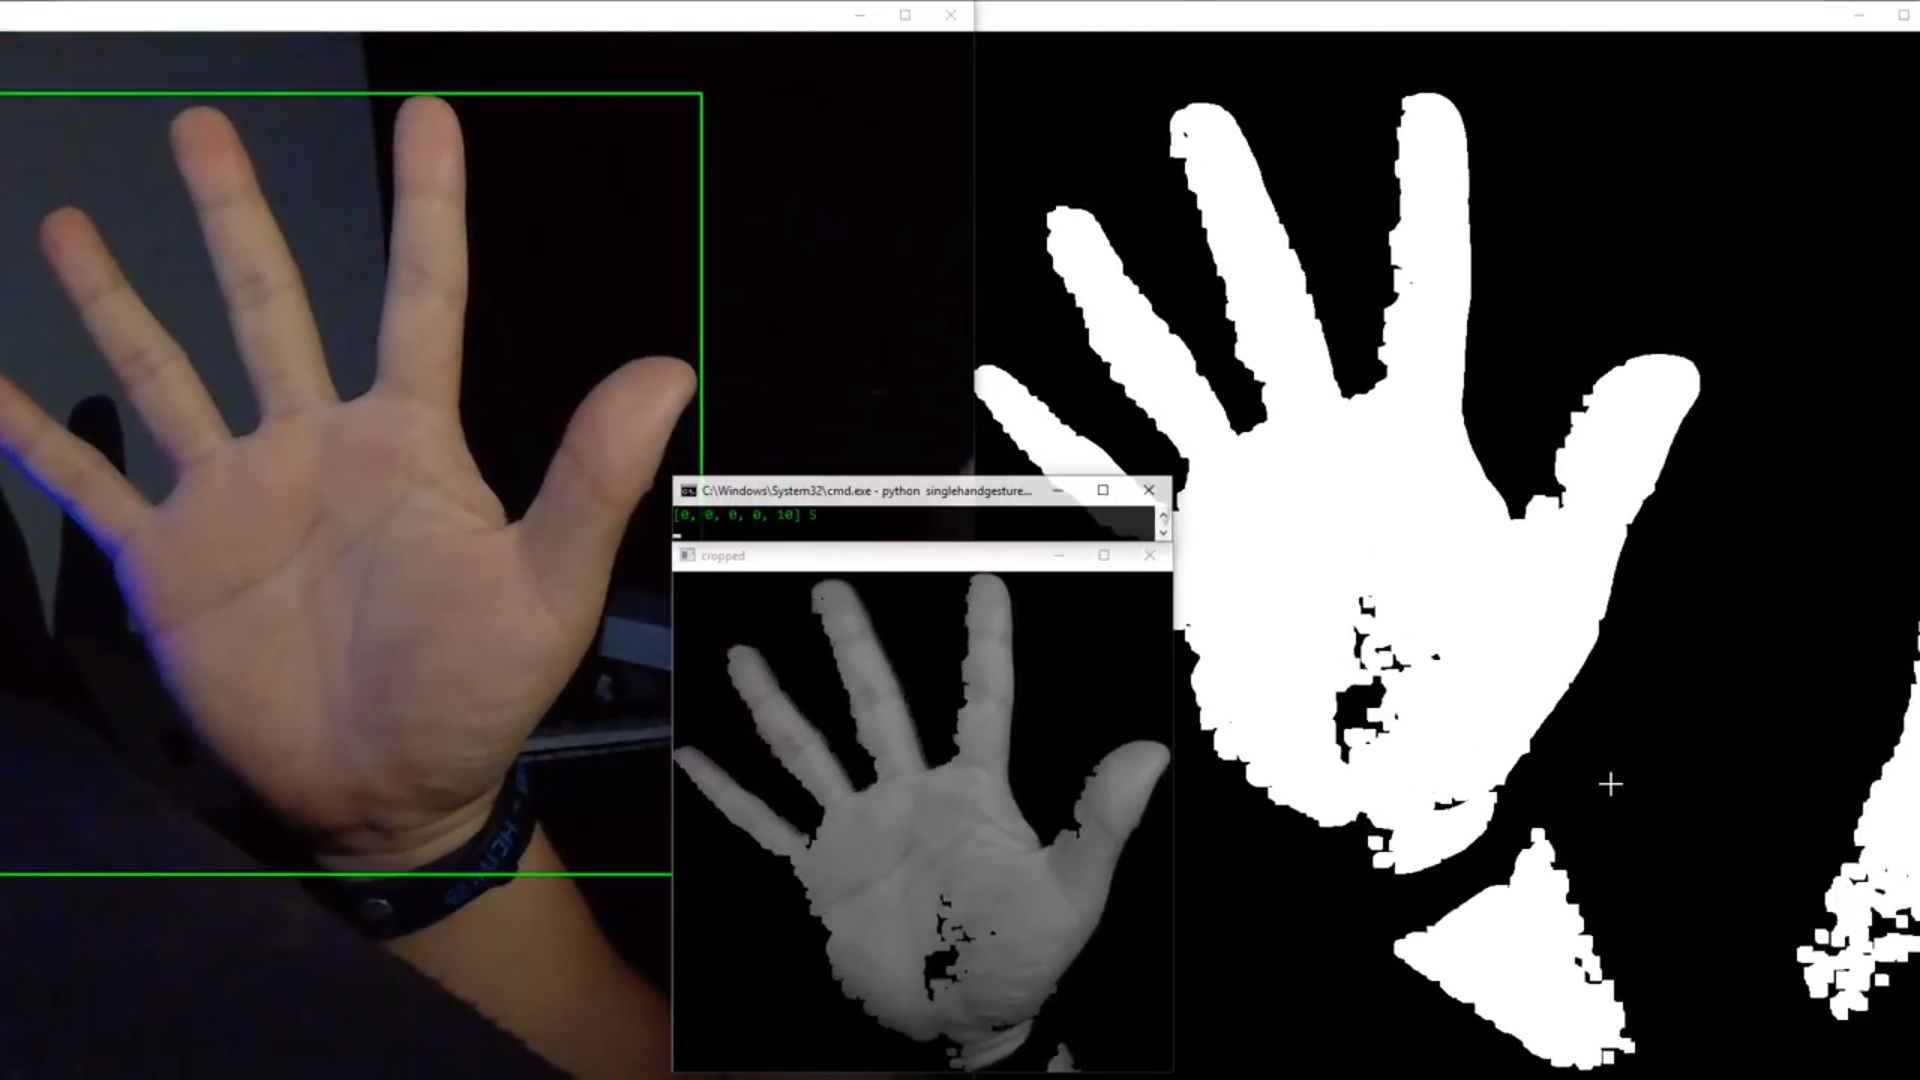
\includegraphics[width=\textwidth]{result_2.png}
\caption{Kết quả khi đưa 5 ngón tay}
\label{fig:foo}
\end{figure}
\section{So sánh}
Ngoài cách làm của chúng tôi là sử dụng máy học thì trên mạng còn \href{https://www.youtube.com/watch?v=H9diqywK6NY}{cách làm khác}. Đó là dùng cách tính các góc giữa khe ngón tay tới đầu ngón tay.
\begin{figure}[!ht]
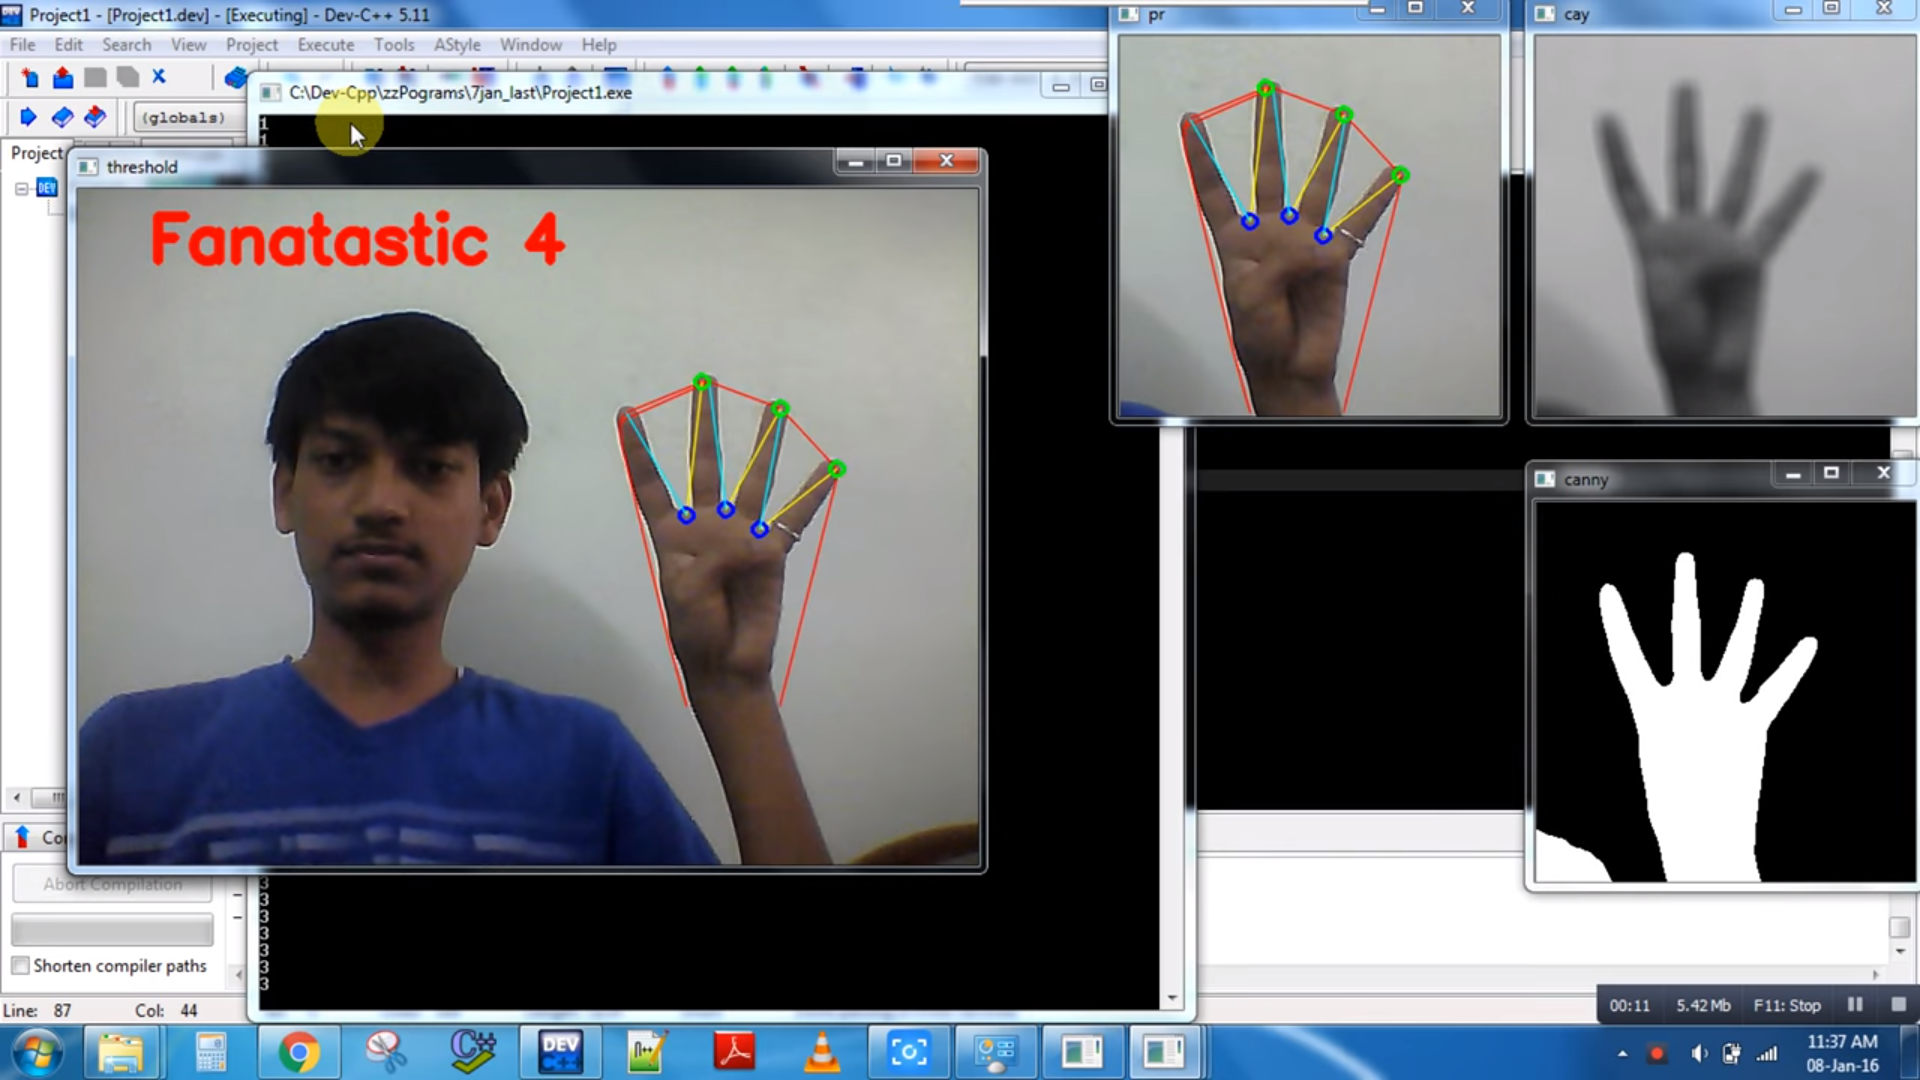
\includegraphics[width=\textwidth]{compare.png}
\caption{Kết quả của cách làm đo góc}
\label{fig:foo}
\end{figure} \\
Và chúng tôi sẽ so sánh cách làm này với cách làm của họ. \\
\begin{center}
\begin{tabularx}{\textwidth}{|c|X|X|}
 \hline
 \thead{So sánh} & \thead{Máy học} & \thead{Đo góc} \\ 
 \hline
 \thead{Ưu điểm} & Thuật toán đơn giản. Có thể làm với nhiều cử chỉ tay với cùng một hướng xử lý
 & Độ chính xác cao với những cử chỉ đã làm.
 \\ 
 \hline
 \thead{Nhược điểm} & Không chính xác bằng, nếu muốn chính xác cần bộ dữ liệu lớn. & Thuật toán phức tạp.
Khó mở rộng để áp dụng với các cử chỉ tay phức tạp
 \\ 
 \hline
\end{tabularx}
\end{center}
\captionof{table}{So sánh giữa 2 cách làm}\label{compare}
\section{Phát triển trong tương lai}
Trong tương lai, chúng tôi sẽ sử dụng camera mà có thể đo khoảng cách để có thể dễ dàng tách được bàn tay ra khỏi mặt người hay cơ thể để tăng độ chính xác và không gây phiền phức thì lúc nào cũng phải cố gắng không để mặt dính vào tay. Thứ hai, chúng tôi sẽ tiếp tục phát triển để có thể xử lý cử chỉ của 2 bàn tay cùng một lúc. Thứ ba, chúng tôi sẽ cho nó học nhiều cử chỉ phức tạp hơn.
\bibliographystyle{unsrt}
\begin{thebibliography}{}
\bibitem{latexcompanion} 
Christos G. Bampis and Jinseok Choi
\textit{\href{http://christosbampis.info/wp-content/uploads/2015/05/DigVidProject_2015.pdf}{Single-hand gesture recognition using image/video processing and machine learning techniques}}.
\bibitem{latexcompanion}
OpenCV
\textit{\href{https://docs.opencv.org/3.2.0/dd/d3b/tutorial_py_svm_opencv.html}{OCR of Hand-written Data using SVM}}.
\bibitem{latexcompanion} 
LearnOpenCV
\textit{\href{https://www.learnopencv.com/histogram-of-oriented-gradients/}{Histogram of Oriented Gradients}}.
\end{thebibliography}

\end{document}